\phantomsection%<---
\chapter{\textit{Mel frequency Capstral Coefficients} (MFCC)}
    \section{Pre-Emphasis}
    Pre-Emphasis merupakan salah satu praktik pra-pemrosesan umum dalam bidang pemrosesan sinyal yang digunakan untuk mengompensasi frekuensi tinggi sinyal yang ditekan selama produksi sinyal. Pra-penekanan merupakan langkah pertama selama adaptasi MFCC, yang dapat diadopsi hanya dengan menerapkan filter high-pass dengan pengaturan [$1, -0.97$]. Proses penyaringan mengubah distribusi energi di seluruh frekuensi, serta tingkat energi keseluruhan. Formula Pre-Emphasis dapat dilihat pada persamaan \ref{eq:pre_emphasis}.
    \begin{equation}
        \hat{y}[n] = x[n] - \alpha \cdot x[n-1]
        \label{eq:pre_emphasis}
    \end{equation}
    Keterangan:
\begin{itemize}
    \item $x[n]$ adalah sinyal input
    \item $\hat{y}[n]$ adalah sinyal keluaran
    \item $\alpha$ adalah faktor pre-emphasis
\end{itemize}
    Keluaran $\hat{y}[n]$ akan menjadi seperti persamaan \ref{eq:sequence}
    \begin{equation}
        \{x(0), x(1) - \alpha x(0), \ldots, x(n-1) - ax(n-2)\}
    \label{eq:sequence}
    \end{equation}

    \section{\textit{Framing} dan \textit{Windowing}}
    Ide di balik pemisahan sinyal menjadi "frame" yang berbeda adalah memecah sinyal data mentah menjadi frame yang sinyalnya cenderung lebih stasioner. Untuk karakteristik akustik yang stabil, suara perlu diperiksa dalam jangka waktu yang cukup singkat. Oleh karena itu, pengukuran spektral jangka pendek biasanya dilakukan selama jendela 20 ms, dan setiap bingkai tumpang tindih 10 ms dengan bingkai berikutnya. Tumpang tindih bingkai sebesar 10 ms memungkinkan karakteristik temporal sinyal audio dilacak. Dengan tumpang tindih bingkai audio, representasi suara akan kira-kira terpusat pada beberapa bingkai.
    Pada setiap frame, jendela diterapkan untuk mempersempit sinyal ke arah batas frame. Secara umum, jendela Hanning dan Hamming \cite{rao2017speech} adalah salah satu metode yang paling banyak digunakan. Jendela ini dapat meningkatkan harmonik, menghaluskan tepi, dan mengurangi efek tepi saat melakukan DFT pada sinyal. Framing dan windowing diterapkan dengan persamaan \ref{eq:framing_and_windowing}.

    \begin{equation}
        x_n[m] = x[n] \cdot w[n]
    \label{eq:framing_and_windowing}
    \end{equation}
Keterangan:
\begin{itemize}
    \item $w[n]$ adalah fungsi windowing
    \item $x_n[m]$ adalah hasil windowing
    \item $x[n]$ adalah sinyal input
\end{itemize}

    \section{\textit{Discrete Fourier Transform} (DFT)}
    \textit{Discrete Fourier Transform} (DFT) banyak digunakan untuk menghitung spektrum daya. Spektrum daya dapat dideskripsikan sebagai distribusi dari daya pada komponen frekuensi pada sinyal \cite{feldman1993power}. Spektrum daya masing-masing frame dapat ditentukan dengan persamaan \ref{eq:dft}.

    \begin{equation}
        X[k] = \sum_{n=0}^{N-1} x[n] \cdot e^{-j2\pi kn/N}
    \label{eq:dft}
    \end{equation}
Keterangan:
\begin{itemize}
    \item $j$ adalah bilangan imajiner
    \item $N$ adalah panjang sinyal
    \item $x[n]$ adalah sinyal input
\end{itemize}

    dengan $x(n)$ adalah sinyal diskrit dan $N$ adalah panjang dari sinyal.
    \section{\textit{Mel-Frequency Filter Bank}}
    \textit{Mel-Frequency Filter Bank} adalah bank filter yang dibangun berdasarkan persepsi nada. Filter Mel awalnya dikembangkan untuk \textit{speech recognition} dan seperti persepsi telinga manusia terhadap ucapan, filter ini menargetkan ekstraksi representasi nonlinier dari sinyal ucapan. \textit{Mel-Frequency Filter Bank} konvensional dibangun dari 40 filter segitiga \cite{YIN2011707}. Fungsi transfer (TF) dari masing-masing filter ke-m dapat dihitung melalui persamaan \ref{eq:mel_filter_bank},

    \begin{equation}
        H_m(k) = 
        \begin{cases} 
            0 & k < f(m-1) \\ 
            \dfrac{k - f(m-1)}{f(m) - f(m-1)} & f(m-1) \leq k < f(m) \\ 
            1 & k = f(m) \\ 
            \dfrac{f(m+1) - k}{f(m+1) - f(m)} & f(m) < k \leq f(m+1) \\ 
            0 & k > f(m+1) 
        \end{cases}
    \label{eq:mel_filter_bank}
    \end{equation}
    dengan $f(m)$ adalah pusat frekuensi dari filter segitiga dan $\Sigma_{m}^{M-1}H_m(k)=1$.
    Skala Mel terhadap frekuensi respons dan sebaliknya dihitung dengan persamaan \ref{eq:m} dan \ref{eq:f}.
    \begin{equation}
        m = 2595 \log_{10} \left( 1 + \frac{f}{700} \right)
    \label{eq:m}
    \end{equation}
    \begin{equation}
        f = 700 \left( 10^{\frac{m}{2595}} - 1 \right)
    \label{eq:f}
    \end{equation}
    Keterangan:
\begin{itemize}
    \item $f$ adalah frekuensi
    \item $m$ adalah skala mel
\end{itemize}
    \section{\textit{Discrete Cosine Transform} (DCT)}
    \textit{Discrete Cosine Transform} (DCT) menyatakan \textit{finite sequence} dari titik data mengenai penjumlahan fungsi kosinus yang berosilasi pada frekuensi yang berbeda. DCT diperkenalkan oleh Nasir Ahmed pada tahun 1972. Dalam proses MFCC, DCT diterapkan pada bank filter Mel untuk memilih koefisien yang paling akurat atau untuk memisahkan hubungan dalam besaran spektral logaritma dari bank filter \cite{strang1999discrete}. DCT dihitung dengan persamaan \ref{eq:dct}

    \begin{equation}
        X_k = \sum_{n=0}^{N-1} x_n \cos\left(\frac{2\pi jnk}{N}\right), \quad k = 0, 1, \ldots, N-1
    \label{eq:dct}
    \end{equation}
    Keterangan:
\begin{itemize}
    \item $x_n$ adalah sinyal diskrit
    \item $N$ adalah panjang sinyal
    \item $X_k$ adalah koefisien MFCC
\end{itemize}

\chapter{Perhitungan \textit{Encoder Cross-Attention}} \label{lampiranD}
\begin{figure}[H]
    \centering
    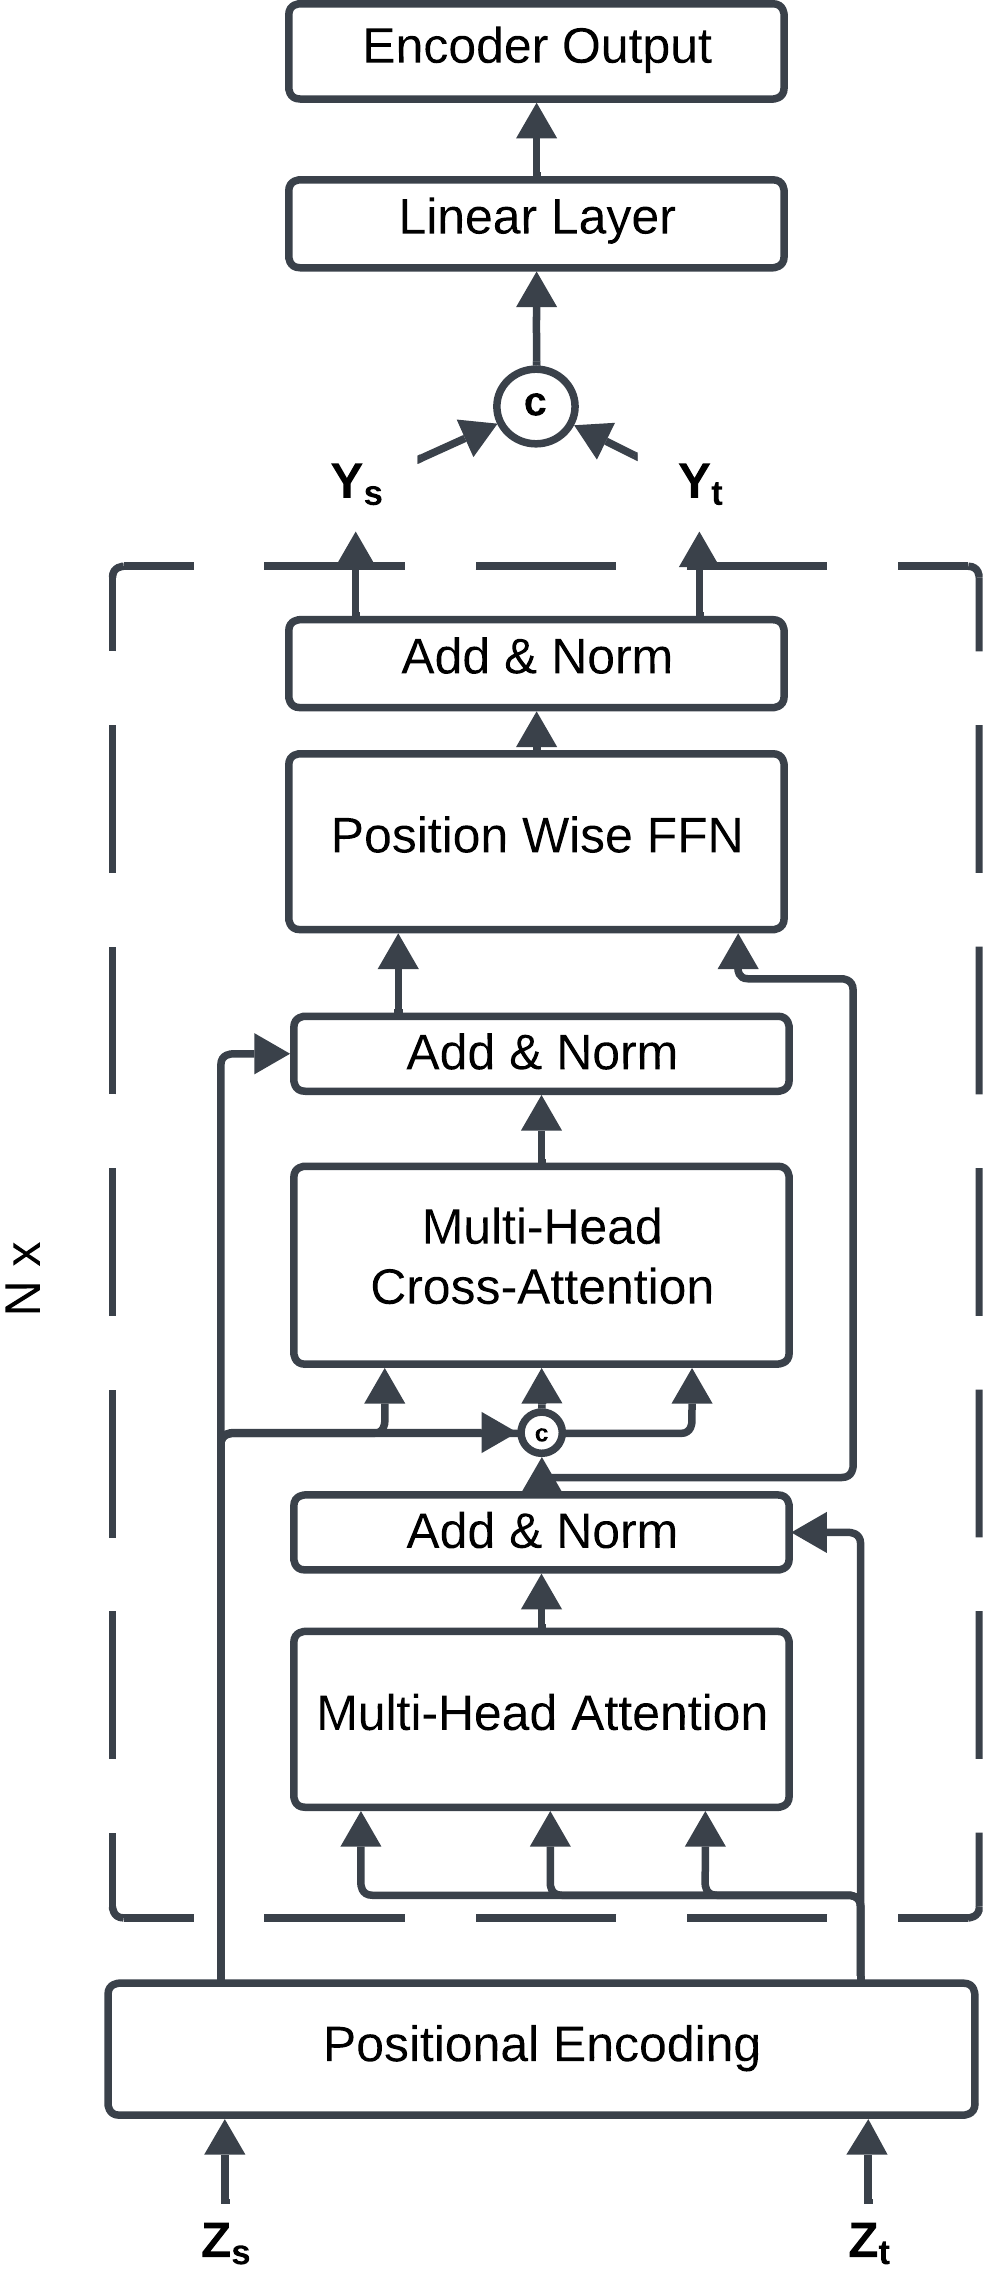
\includegraphics[width=0.4\linewidth]{gambar/Transformer Encoder.png}
    \caption{Encoder Cross Attention}
    \label{fig:crosss-attention}
\end{figure}

    \section{\textit{Self-Attention} dan \textit{Multi-Head Attention}}
     Proses dari \textit{Self-Attention} atau yang memiliki nama lain \textit{Scaled Dot-Product Attention} dapat dilihat pada Gambar \ref{fig:self_attention}.
\begin{figure}[H]
    \centering
    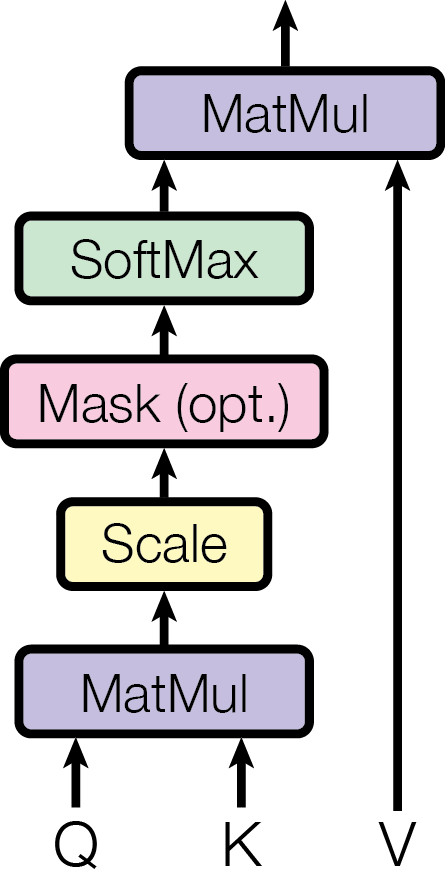
\includegraphics[width=0.25\linewidth]{gambar/ModalNet-19.png}
    \caption{\textit{Self-Attention} atau \textit{Scaled Dot-Product Attention}}
    \label{fig:self_attention}
\end{figure}

Proses dari \textit{Multi-Head Attention} dapat dilihat pada Gambar \ref{fig:multi_head_attention}.
\begin{figure}[H]
    \centering
    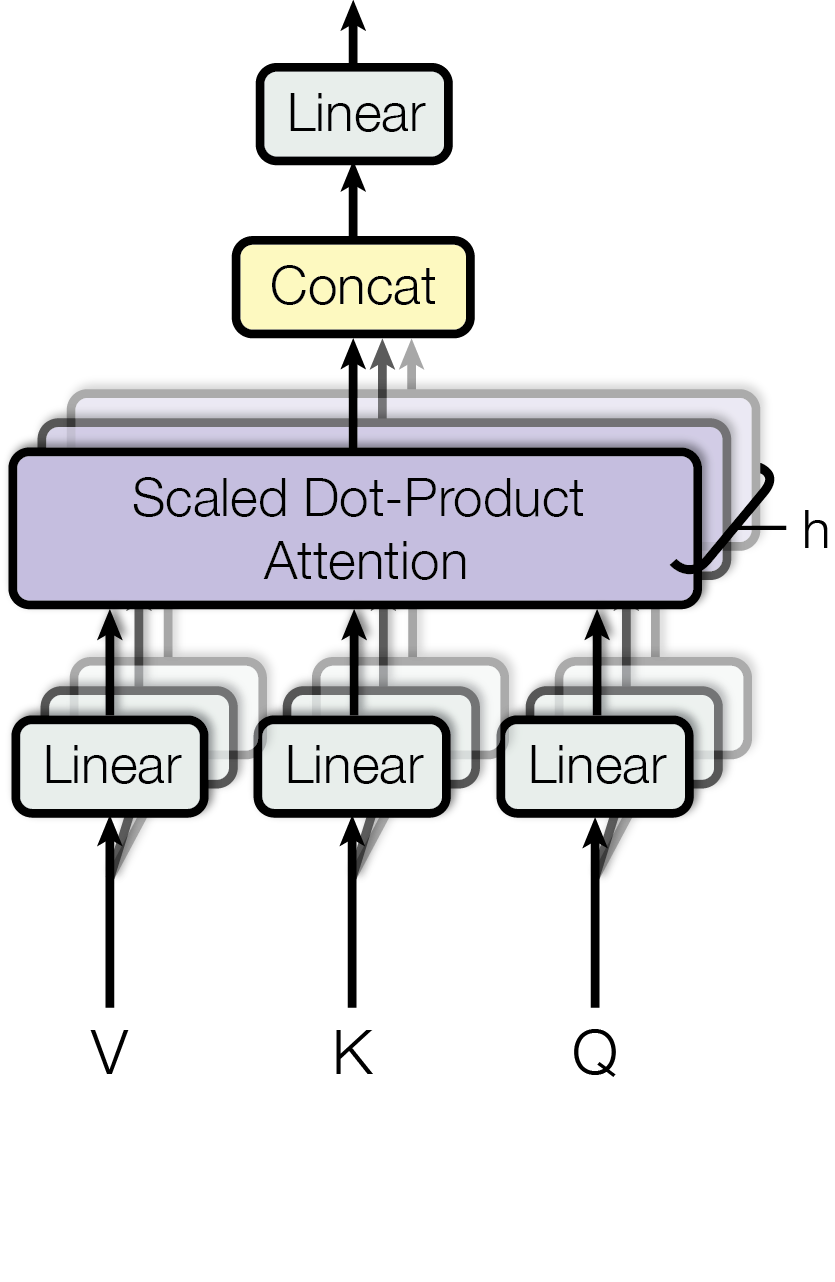
\includegraphics[width=0.38\linewidth]{gambar/ModalNet-20.png}
    \caption{\textit{Multi-Head Attention}}
    \label{fig:multi_head_attention}
\end{figure}

Inisiasi nilai variabel diperlukan untuk penentuan nilai awal pada pelatihan. Nilai yang digunakan adalah nilai yang sama dengan paper \textit{"Attention Is All You Need"} dengan beberapa penyesuaian \cite{vaswani2023attentionneed}. Nilai variabel inisiasi dapat dilihat pada tabel \ref{tab:transformer_encoder_vars}.
\begin{table}[H]
    \centering
    \caption{Tabel Variabel untuk Encoder Transformator}
    \begin{tabular}{l c}
        \hline
        \textbf{Nama Variabel} & \textbf{Nilai Variabel} \\ \hline
        EMBED\_DIM & 64 \\ \hline
        SEQ\_LENGTH & 512 \\ \hline
        NUM\_FEATURE & 8 \\ \hline
        D\_MODELS & 8 \\ \hline
        NUM\_HEADS & 8 \\ \hline
        DROPOUT\_RATE & 0.2 \\ \hline
        EPOCHS & 30 \\ \hline
    \end{tabular}
    \label{tab:transformer_encoder_vars}
\end{table}

Matriks fitur riwayat pasien $Z_t$ berukuran $8\times1$ dimasukkan ke dalam layer linear agar memiliki dimensi yang sama dengan matriks hasil ekstraksi fitur MFCC sehingga memiliki ukuran $8\times64$. Matriks fitur suara $Z_s$ hasil ekstraksi fitur MFCC berukuran $512\times64$ dan matriks fitur riwayat pasien berukuran $8\times64$ ditambahkan dengan token [cls] menjadi masing-masing berukuran $513\times64$ dan $9\times64$.

Matriks fitur riwayat pasien lalu masuk ke dalam mekanisme \textit{Multi-Head Attention} dan \textit{Layer Norm} dengan hasil matriks berukuran $9\times64$. Matriks ini selanjutnya di \textit{concat} dengan matriks fitur suara yang telah ditambah token [cls] berukuran $513\times64$ sehingga menghasilkan matriks berukuran $521\times64$.

Matriks fitur suara yang telah di \textit{concat} dengan matriks fitur riwayat pasien yang telah melalui mekanisme \textit{Multi-Head Attention} lalu masuk ke dalam mekanisme \textit{Multi-Head Cross Attention}. Operasi yang digunakan pada \textit{Multi-Head Cross Attention} sama dengan \textit{Multi-Head Attention}, perbedaannya terletak pada input berupa gabungan antara fitur suara dan fitur riwayat pasien. Setelah melewati \textit{Layer Norm} ukuran matriks hasil \textit{Multi-Head Cross Attention} menjadi $513\times64$.

\section{\textit{Feed-Forward Network}}
Matriks hasil \textit{Multi-Head Attention} dan \textit{Multi-Head Cross Attention} masing-masing masuk ke dalam mekanisme \textit{Feed-Forward Network}. mekanisme \textit{Feed-Forward Network} terdiri dari tiga operasi utama yaitu \textit{Linear Transformation}, \textit{Activation Function} dan \textit{Layer Normalization}. Transformasi Linear diimplementasikan sebagai \textit{fully connented layer}, atau juga dikenal sebagai \textit{dense layer}, yang menghubungkan setiap neuron masukan ke setiap neuron keluaran. Langkah berikutnya dalam operasi \textit{Feed-Forward Network} adalah menerapkan fungsi aktivasi. Fungsi ini merupakan fungsi non-linier yang memungkinkannya mempelajari pola yang lebih kompleks. Fungsi aktivasi yang digunakan pada model ini adalah GELU (\textit{Gaussian Error  Linear Unit}) yang memiliki kecepatan dan konvergensi yang lebih baik karena telah menggabungkan properti dari dropout, zoneout, dan ReLUs \cite{hendrycks2023gaussianerrorlinearunits}. Persamaan fungsi aktivasi GELU dapat dilihat pada persamaan \ref{eq:gelu}.

\begin{equation}
    \text{GELU}(x) = x P(X \leq x) = x \Phi(x) = x \cdot \frac{1}{2} \left[ 1 + \operatorname{erf}(x / \sqrt{2}) \right]
    \label{eq:gelu}
\end{equation}

Fungsi aktivasi GELU dapat diaproksimasi dengan persamaan \ref{eq:approx_gelu_1}
\begin{equation}
    0.5x(1 + \tanh[\sqrt{2/\pi}(x + 0.044715x^3)])
    \label{eq:approx_gelu_1}
\end{equation}
atau persamaan \ref{eq:approx_gelu_2}.
\begin{equation}
    x\sigma(1.702x)
    \label{eq:approx_gelu_2}
\end{equation}

Tahap terakhir pada \textit{Feed-Forward Network} adalah \textit{Layer Normalization}. \textit{Layer Normalization} adalah teknik yang menormalkan masukan di seluruh dimensi fitur (bukan dimensi batch), menstabilkan jaringan dan mempercepat pelatihan. Output dari \textit{Feed-Forward Network} berupa kedua matriks dengan ukuran $513\times64$ dan $9\times64$.

\section{Output Encoder $Y_s$ dan $Y_t$}
Proses dari keseluruhan di atas merupakan proses dalam satu blok encoder, proses ini diulang sebanyak N\_BLOCK. Didapatkan vektor $Y_s$ dan $Y_t$ dengan ukuran $1\times64$ yang kemudian di \textit{concat} secara horizontal/kolom sehingga didapatkan vektor berukuran $1\times128$. Vektor ini kemudian masuk ke dalam fungsi aktivasi GELU dan layer Linear sehingga didapatkan vektor berukuran $1\times64$. Fungsi aktivasi Softmax digunakan untuk mengakomodir klasifikasi multi-kelas dengan menghasilkan probabilitas setiap kelas dengan jumlah semua probabilitas berjumlah tepat 1. Fungsi aktivasi Softmax dapat dilihat pada persamaan \ref{eq:softmax}.
% Requires: \usepackage{amsmath}
\begin{equation}
    \sigma(\mathbf{z})_i = \frac{e^{z_i}}{\sum_{j=1}^{K} e^{z_j}}, \quad \text{for } i = 1, \ldots, K
    \label{eq:softmax}
\end{equation}
Keterangan:
\begin{itemize}
    \item $\sigma$ adalah softmax
    \item $\mathbf{z}$ adalah input vektor
    \item $K$ adalah jumlah kelas
    \item $e^{z_i}$ fungsi eksponensial untuk vektor input
    \item $e^{z_j}$ fungsi eksponensial untuk vektor output
\end{itemize}
Fungsi \ref{eq:softmax} menghasilkan vektor $1\times3$ yang berisi nilai probabilitas dari ketiga kelas. Nilai probabilitas terbesar menunjukkan prediksi kelas dari data.

\phantomsection%<---
\chapter{\textit{Optimizer Adam}} \label{lam:lampiran_a}
    \section{Optimizer Adam pada Transformers}
    Adam menggabungkan kelebihan dari dua algoritma optimisasi yaitu momentum dan RMSProp dengan mengestimasi rata-rata dan varians dari gradien. Dalam model Transformers, parameter $\theta$ mencakup bobot dan bias untuk:
\begin{itemize}
    \item Lapisan \textit{self-attention} dan \textit{multi-head attention} (seperti bobot proyeksi query, key dan value).
    \item \textit{Feed-Forward Network}.
    \item Parameter \textit{Layer Normalization}.
\end{itemize}
Setiap parameter diperbarui menggunakan persamaan di bawah.

\subsection{Persamaan Oprimizer Adam}

1. Menghitung gradien dari loss \( L \) dengan parameter \( \theta \) dengan persamaan \ref{eq:gradien_loss}:
\begin{equation}
    g_t = \nabla_{\theta} L(\theta_t)
    \label{eq:gradien_loss}
\end{equation}

2. Perbarui estimasi momentum bias dengan persamaan \ref{eq:mean_gradien}dan \ref{eq:varian_gradien}:
\begin{equation}
    m_t = \beta_1 m_{t-1} + (1 - \beta_1) g_t
    \label{eq:mean_gradien}
\end{equation}
\begin{equation}
    v_t = \beta_2 v_{t-1} + (1 - \beta_2) g_t^2
    \label{eq:varian_gradien}
\end{equation}

3. Terapkan koreksi bias pada momentum dengan persamaan \ref{eq:bias_correction}:
\begin{equation}
    \hat{m}_t = \frac{m_t}{1 - \beta_1^t}, \quad \hat{v}_t = \frac{v_t}{1 - \beta_2^t}
    \label{eq:bias_correction}
\end{equation}
4. Perbarui parameter dengan persamaan \ref{eq:update_param}:
\begin{equation}
    \theta_{t+1} = \theta_t - \eta \frac{\hat{m}_t}{\sqrt{\hat{v}_t} + \epsilon}
    \label{eq:update_param}
\end{equation}
Keterangan:
\begin{itemize}
    \item $g_t$ adalah fungsi gradien
    \item $L(\theta_t)$ adalah fungsi Loss
    \item $m_t$ adalah momentum
    \item $v_t$ adalah velocity
    \item $\eta$ merupakan \textit{learning rate}.
    \item $\beta_1$ dan $\beta_2$ adalah \textit{hyperparameter} yang mengendalikan tingkat peluruhan estimasi momen.
    \item $\epsilon$ adalah konstanta kecil untuk mencegah pembagian dengan nol.
\end{itemize}


\subsection{Contoh Perhitungan}
Asumsikan :

\begin{itemize}
  \item Learning rate $\eta = 0.001$,
  \item $\beta_1 = 0.9$, $\beta_2 = 0.999$,
  \item $\epsilon = 10^{-8}$,
  \item Gradien pada \textit{timestep} $t$: $g_t = 0.02$,
  \item Estimasi momentum sebelumnya: $m_{t-1} = 0.01$, $v_{t-1} = 0.0001$,
  \item $t = 10$.
\end{itemize}


Langkah-langkah perhitungan:

1. Hitung estimasi momen bias:
\[
m_t = \beta_1 m_{t-1} + (1 - \beta_1) g_t = 0.9 \cdot 0.01 + (1 - 0.9) \cdot 0.02 = 0.011
\]
\[
v_t = \beta_2 v_{t-1} + (1 - \beta_2) g_t^2 = 0.999 \cdot 0.0001 + (1 - 0.999) \cdot (0.02)^2 = 0.0001004
\]

2. Terapkan koreksi bias:
\[
\hat{m}_t = \frac{m_t}{1 - \beta_1^t} = \frac{0.011}{1 - 0.9^{10}} \approx 0.0111
\]
\[
\hat{v}_t = \frac{v_t}{1 - \beta_2^t} = \frac{0.0001004}{1 - 0.999^{10}} \approx 0.000102
\]

3. Hitung pembaruan parameter:
\[
\Delta \theta = \eta \frac{\hat{m}_t}{\sqrt{\hat{v}_t} + \epsilon}
\]
Subsitusikan nilai:
\[
\Delta \theta = 0.001 \cdot \frac{0.0111}{\sqrt{0.000102} + 10^{-8}} \approx 0.00109
\]

4. Perbarui parameter:
\[
\theta_{t+1} = \theta_t - \Delta \theta
\]

\phantomsection%<---
\chapter{Variasi Model dan \textit{Hyperparameter Tuning}} \label{lampiran B}
 \begin{table}[ht]
    \centering
    \caption{Variasi Model dan Hyperparameter Transformer}
    \begin{tabular}{@{}lcc@{}}
        \toprule
        \textbf{Hyperparameter} & \textbf{Small Model} & \textbf{Big Model} \\ \midrule
        Jumlah Layer/Blok Encoder ($N\_BLOCK$)      & 6                   & 12                 \\
        Dimensi Embedding ($d_\text{model}$) & 64                 & 128               \\
        Dimensi Feedforward ($d_\text{ff}$) & 256                & 512               \\
        Jumlah Head Attention  & 8                   & 16                 \\
        Dropout                & 0.2                 & 0.3                \\
        Batch Size             & 32                  & 64                \\
        Learning Rate          & 1e-4                & 5e-5               \\ \bottomrule
    \end{tabular}
    \label{tab:transformer-variations}
\end{table}